\documentclass{beamer}
\usepackage{lsfolien,enumitem}
\usepackage[english]{babel}
\setlist[itemize]{noitemsep,label={\color{blue}$\rhd$}}
           
\myfootline{Sustainability, Environment, Management -- Winter Term
  2021}{Hans-Gert Gr\"abe}

\newcommand{\ueberschrift}[1]{\begin{center}\bf #1\end{center}}

\parskip1em

\title{Supply Chains and SCOR as Reference Model}

\subtitle{Research Seminar in the Module 10-202-2309\\ for Master Computer
  Science}

\author{Prof. Dr. Hans-Gert Gräbe\\
\url{http://www.informatik.uni-leipzig.de/~graebe}}

\date{November 2021}
\begin{document}

{\setbeamertemplate{footline}{}
\begin{frame}
  \titlepage
\end{frame}}

\begin{frame}{Systemic Structure of (Enterprise) Organisations}

The systemic understanding of an (entreprise) organisation, which can be read
off from the normative documents (APQC-PCF) and practically relevant
enterprise modelling (Business TRIZ) examined so far, assumes two systemic
levels to be distinguished -- \textbf{operational} and \textbf{strategic}
management.

From the \textbf{perspective of strategic management}, the system is the whole
enterprise, divided into strategic business units as components (APQC-PCF
levels \emph{category} and \emph{process group}).

APQC-PCF provides here for a company-wide division into 13 \emph{categories}
as strategic business areas.
\end{frame}

\begin{frame}{Systemic Structure of (Enterprise) Organisations}

The focus of \textbf{operational management} is on the concrete design and
development of these individual business areas at the operational and thus at
an intrinsically shorter time horizon.

APQC postulates at that level clearly more centralised management structures
with corresponding authorisations and rights of intervention, but also
responsibilities.

On the other hand, it also provides for differently designed intra-company
structures through \emph{variants of the standard} at the level of modelling
processes, activities and tasks.
\end{frame}

\begin{frame}{Systemic Structure of (Enterprise) Organisations}

These standardisation efforts are thus directed at the \emph{strategic
  structural level} and a certain standardisation of \emph{operational
  processes in their methodological meta-model} rather than structural model
dimension.

Organise the comparison between process planning and real-world process
execution as a contradiction between \emph{justified expectations} and
\emph{experienced results} in a comparable way by regularly recording
\emph{Key Perfomance Indices} (KPI) (see 13.6 \emph{Measure and Benchmark} in
APQC-PCF).

\end{frame}

\begin{frame}{Systemic Structure of (Enterprise) Organisations}

This information is part of a \emph{global conceptualisation} at this
subsystem level, of a \emph{cooperative world view} as an emergent phenomenon,
which is inseparably linked to the development and strenghtening of the
structure at this subsystem level.

Even if the KPIs are modelled and collected globally throughout the company,
the possible uses of these instruments remain the same at the operational
level, because the authorisation of the operational management is limited
accordingly and thus \emph{judgement practices} can be executed only within
the subsystem. 
\end{frame}

\begin{frame}{Systemic Structure of (Enterprise) Organisations}

In agile contexts with instruments of indirect control there are often more
than two such system levels to distinguish, which can be read off from clearly
differing time horizons.  In Scrum, for example, the structuring units
\emph{Daily Scrum}, \emph{Sprint} and \emph{Product Backlog} or \emph{Project}
mark four systemic contexts -- the \emph{Project} as a whole as a component of
strategic corporate development, the individual \emph{Sprints} as components
of the system \emph{Project}, the contents of which are negotiated between the
project owner as control component in the \emph{system Project} and the team,
and the agile implementation structures in the \emph{system Sprint} by the
individual team members as components (or resources?) with, e.g., their
progress reports in the \emph{Daily Scrum}.
\end{frame}

\begin{frame}{Systemic Structure and Agent Based Systems}

Most management theories do not say much about the issues
\begin{itemize}
\item maintenance of the emergent systemic resources as \emph{infrastructure}
  and 
\item development of a \emph{cooperative world view}
\end{itemize}
at the strategic level of the company. One of the (non-explicit) preconditions
at that level seems to be a certain collective decision-making, since the
managers involved represent different operational areas that are all important
by their own, representing, in addition to \emph{goals} as justified
expectations, the various intrinsic logics of the operational areas.

\end{frame}

\begin{frame}{Systemic Structure and Agent Based Systems}

A radical answer to this problem is the transition to agent-based systems as
presented in the seminar in the previous week. A system is built from agents
as components whose internal reproduction conditions (\enquote{belief,
  knowledge, desire, obligation, commitment, state, thinking about past
  actions, learning, (internal) goals} -- Slide~9) are decisive for what kind
of systems can be assembled from them at all.

Goals or objectives of an overall system no longer seem to drive the
development, but (solely?) the coordination achieved by
\enquote{communication, negotiation, information sharing} (Slide~34) among the
agents as system components.

However, later (Slide~35) a CEO with \enquote{guidance} appears.

\end{frame}

\begin{frame}{Systemic Structure and Agent Based Systems}

Essential \enquote{advantages of an agent-based approach in business
  environments} are summarised on Slide~37:
\begin{itemize}
\item Head business management focuses on higher-level decisions.
\item Improved problem-solving capabilities through specialisation.
\item Improved problem-solving capabilities through mutual support.
\item Sophisticated goal-oriented communication.
\item Improved physical organisation.
\item Outsourcing of cross-cutting concerns.
\end{itemize}

\end{frame}

\begin{frame}{Systemic Structure and Agent Based Systems}

Hence, other aspects than the seeming ability of agents to act autonomously
and the assertion that a separate optimisation of the agents leads to
optimality of the overall system come to the front. These are primarily
\enquote{beliefs} and \enquote{knowledge} as two properties of an
\textbf{emergent system-specific conceptual system} -- a \enquote{cooperative
  world view} -- which allows to capture in language form the specific
\enquote{reduction to essentials} of the system-internal relations between the
components.

The temporal offset of the unfolding of conceptual systems at different levels
is an essential characteristic of dynamics in systemic structures.

\end{frame}

\begin{frame}{Systemic Structure and Agent Based Systems}

In an agent-based approach the existence of such a (developed) conceptual
system is \textbf{postulated} for the agents as components.

But it must also \emph{unfold at the level of the system}. In view of the
reduction of the component properties to their specification, the conceptual
systems of the components enter into this new systemic conceptual system only
in a reduced form, but must be expanded by conceptualisations and modelling
approaches for the essential interactions between the components.
\end{frame}

\begin{frame}{A Market-based Landscape of Independent Producers}

Agent-based systems model a basic assumption of the free market concept -- the
contract-based action of economic subjects as homines oeconomici optimising
private benefits leads to an optimal overall economic system by the
\enquote{blind action of the market}.

This belief is in apparent contradiction not only to the importance of
institutionalised procedures in the \textbf{concept of technology} developed
in the lecture, but also to all \textbf{practical} efforts to standardise
business processes, which were addressed in two seminar presentations
(APQC-PCF and Business TRIZ).

Production based on the division of labour is only possible if this division
of labour is embedded in overarching institutionalisation processes, based on
common conceptual systems which accompany the exchange of (meaningful for both
parties) labour products and services between independent third parties.

\end{frame}

\begin{frame}{Supply Chain Management}

The exchange of products and services across company boundaries is not only
oriented towards the induced money flows, but also towards the material
properties -- the \emph{use value} -- of the exchange products. The more
detailed the corresponding conceptual systems for qualitative and quantitative
parameters of the exchange products are developed, the more precisely these
use value can be described.

\textbf{Product quality} and \textbf{process quality} -- capability of a
company not only to produce qualitatively adequate products, but do deliver
them in predictable time and cost frames and offer required services during
the use of the products in the operation by third parties.

\textbf{Supply chain management} focuses on such issues of assessing quality
capability in supply chains.
  
\end{frame}

\begin{frame}{SCOR as Supply Chain Operations Reference Model}

Similar to APQC-PCF, SCOR as a \emph{reference model} systematises the
essential aspects that have to be considered in a structured way during such
an assessment of partners in the supply chain.

SCOR 1.0 was released in 1996 and has since been developed in various
versions.

Today, the further development of SCOR is coordinated by the ASCM Foundation
-- the \emph{Association for Supply Chain Management}.
  
\end{frame}

\begin{frame}{SCOR as Supply Chain Operations Reference Model}

In its focus are 
\begin{itemize}
\item definitions of \textbf{key performance indicators} that balance
  customer requirements with internal capabilities,
\item the architecture of \textbf{processes} to leverage the technology,
\item the adoption of \textbf{practices} that are more than just white papers,
\item and development of \textbf{people} to have both the knowledge and skills
  to make it all happen with required performance to achieve the promised RoI.
\end{itemize}
\end{frame}

\begin{frame}{SCOR as Supply Chain Operations Reference Model}

SCOR as the standard process reference model for supply-chain management
brings order to the diverse activities that make up the supply chain, and
provides common terminology and standard process descriptions.

The model allows companies to:
\begin{itemize}
\item evaluate their own processes effectively;
\item compare their performance with other companies both within and outside
  their industry segment;
\item pursue specific competitive advantages;
\item use benchmarking and best practice information to prioritise their
  activities;
\item quantify the benefits of implementing change; and
\item identify software tools best suited to their specific process
  requirements.
\end{itemize}

\end{frame}

\begin{frame}{SCOR as Supply Chain Operations Reference Model}

\begin{center}
  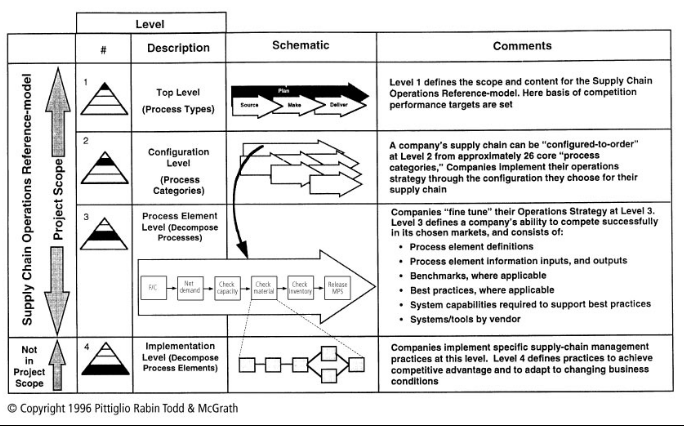
\includegraphics[width=.9\textwidth]{images/Stewart-1997.png}\\
  The four level model of SCOR as displayed in (Stewart 1997)
\end{center}

\end{frame}

\begin{frame}{SCOR as Supply Chain Operations Reference Model}
SCOR focuses on four basic supply-chain processes as \textbf{top level process
  types}, defining the scope and overall content of the SCOR model, and 26
\textbf{core process categories} sorted in 12 groups as possible components of
a supply chain.

\begin{minipage}[t]{.45\textwidth}\small\raggedright
\begin{itemize}
\item[(1)] \textbf{Plan} with
  \begin{itemize}[leftmargin=0pt]
  \item \emph{Demand/supply planning}.
  \item \emph{Infrastructure planning}. 
  \end{itemize}
\item[(2)] \textbf{Source} with
  \begin{itemize}[leftmargin=0pt]
  \item \emph{Sourcing/material acquisition}.
  \item \emph{Source infrastructure}.  
  \end{itemize}
\item[(3)] \textbf{Make} with
  \begin{itemize}[leftmargin=0pt]
  \item \emph{Production execution}.
  \item \emph{Make infrastructure}. 
  \end{itemize}
\end{itemize}
\end{minipage}\hfill
\begin{minipage}[t]{.45\textwidth}\small\raggedright
\begin{itemize}
\item[(4)] \textbf{Deliver} with
  \begin{itemize}[leftmargin=0pt]
  \item \emph{Demand management}.
  \item \emph{Order management}.
  \item \emph{Warehouse management}.
  \item \emph{Transportation management}.
  \item \emph{Installation management}.
  \item \emph{Deliver infrastructure}.
  \end{itemize}
\end{itemize}
\end{minipage}
\end{frame}

\begin{frame}{SCOR as Supply Chain Operations Reference Model}

\begin{itemize}
\item SCOR is designed to be used in \textbf{change management processes}.
\item SCOR \textbf{creates goals and measures} against industry best
  practices.
\item SCOR allows to estimate the financial costs and return on
  \textbf{specific improvements}.
\item SCOR \textbf{requires} the existence of a \textbf{comprehensive
  operations strategy} which is well understood by the entire management team
  and is consistent with the \textbf{company's overall business strategy}.
\item SCOR supports \textbf{selective priorisation} of practical
  implementations based on strategic importance.
\item SCOR aims at supporting the business strategy, rapid decision making,
  facilitation by appropriate support systems and information technologies.  
\end{itemize}
  
\end{frame}




\end{document}
